\setcounter{section}{3}

\graphicspath{{lectures/3Analytic/asy/}}

\setcounter{subsection}{3}
\subsection*{The Extended Complex Plane and the Riemann Sphere: non-examinable}

\begin{defn}
The \emph{extended complex plane} is the set $\cl\C=\C\cup\{\infty\}$ consisting of the complex numbers together with a \emph{point at infinity.}
\end{defn}

The point at infinity can be thought of as the limit of any sequence of complex numbers whose modulus grows unboundedly. It can also be considered as a way of making \emph{rational functions} behave nicely: for example
\[f:\cl\C\to\cl\C:z\mapsto \frac 1{z-2}\]
is \emph{bijective}, if we do the natural thing by taking $f(2)=\infty$ and $f(\infty)=0$. 

\begin{defn}
The \emph{Riemann sphere} $S^2$ is the unit sphere identified with $\cl\C$ via a \emph{stereographic projection}
\[P:S^2\to\cl\C\]
as shown in the picture. Let $N=(0,0,1)$ be the north pole of the sphere and identify $\C$ with the equatorial plane: $(x,y,0)\leftrightsquigarrow x+iy$. 
\begin{itemize}
  \item If $\zeta\in S^2\setminus\{N\}$ then $P(\zeta)$ is the intersection of the line through $N$ and $\zeta$ with $\C$.
  \item Define $P(N)=\infty$.
\end{itemize}
\end{defn}

\begin{center}
\includemedia[ %transparent=true, 
 %activate=onclick,
 add3Djscript=asylabels.js,
 %add3Djscript=3Dspintool.js,
 3Dmenu,
  3Dcoo=3.82 -0.13 -15.78,
  3Dc2c=0.97 -0.19 0.17,
  3Droo=400,
  3Droll=0.2,
 3Dlights=Headlamp]{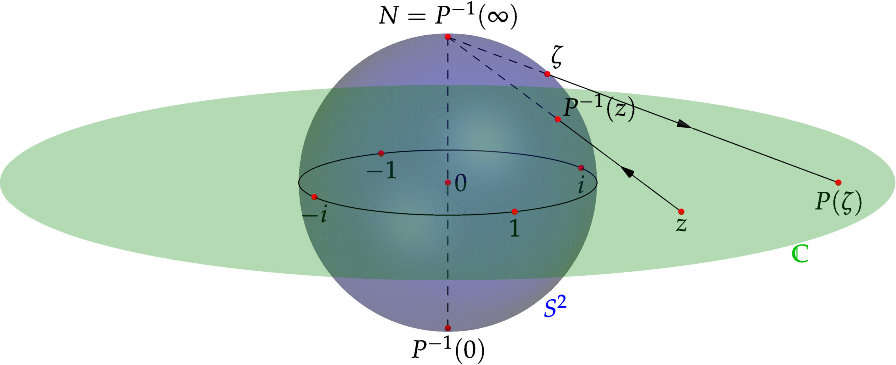
\includegraphics{complex-stereo+0_0}}{complex-stereo+0.prc}
\end{center}

% The Riemann sphere has many applications, including:
% \begin{itemize}
%   \item To perform calculations in \emph{spherical geometry} using simpler manipulations of the plane.
%   \item The visualization of the complex plane work with the extended complex plane in such a way that the point at infinity can be visualized.
% \end{itemize}

\begin{thm}
The stereographic projection is a bijective function $P:S^2\to\cl\C$. For explicit formulæ,  if $\zeta=(X,Y,Z)\in S^2\setminus\{N\}$, and $z=x+iy\in \C$, then
\[P(\zeta)=\frac 1{1-Z}(X,Y,0)\qquad\text{and}\qquad P^{-1}(z)=\left(\frac{2x}{\nm z^2+1},\frac{2y}{\nm z^2+1},\frac{\nm z^2-1}{\nm z^2+1}\right)\]
Moreover, the stereographic projection is infinitely differentiable (away from the north pole).
\end{thm}

\begin{proof}
First observe that all points on the line joining the north pole and $(x,y,0)$ have the form
\[(X,Y,Z)=(1-t)(0,0,1)+t\bigl(x,y,0\bigr)\]
for some real $t$. This lies on the sphere if and only if $X^2+Y^2+Z^2=1$: i.e.
\[(1-t)^2+t^2\nm{z}^2=1\iff t\left((\nm z^2+1)t-2\right)=0\]
The north pole $N$ corresponds to $t=0$, while $t=\frac 2{\nm z^2+1}$ yields the expression for $P^{-1}(z)$.\\
It is now straightforward to check that the expression for $P(\zeta)$ really is the inverse of $P^{-1}(z)$. We therefore have a bijective correspondence $S^2\setminus\{N\}\to\C$. Identifying the north pole with $\infty$ makes the full correspondence $P:S^2\to\cl\C$ a bijection.\\
Differentiability is immediate, since both $P$ and $P^{-1}$ are rational functions which never have zero denominator ($1-Z=0\iff Z=1\iff \zeta=N$).
\end{proof}


There are many nice features of the stereographic projection. In particular:
\begin{thm}
\begin{enumerate}
  \item The projection is \emph{conformal}: two curves in $S^2$ meet at an angle $\alpha$ if and only if their projections to $\cl\C$ also meet at the same angle. This is important for differential geometry.
  \item Rational points on $S^2\setminus\{N\}$ correspond to rational points in $\C$: $X,Y,Z\in\Q\iff x,y\in\Q$. This is important for number theory.
  \item Circles in $S^2$ correspond to circles or straight lines in $\C$ (a line may be thought of as a circle through $\infty$).
\end{enumerate}
\end{thm}


\begin{minipage}[t]{0.5\linewidth}\vspace{0pt}
The proofs are left as exercises: all are elementary, if a little algebraically tortuous! Proving part 1 will certainly require a solid refresher of multivariable calculus\ldots\\

\end{minipage}\begin{minipage}[t]{0.5\linewidth}\vspace{0pt}
\flushright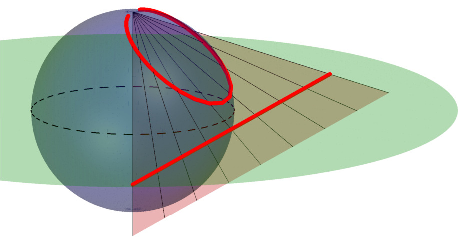
\includegraphics{complex-stereocircle3}
\end{minipage}

\begin{center}
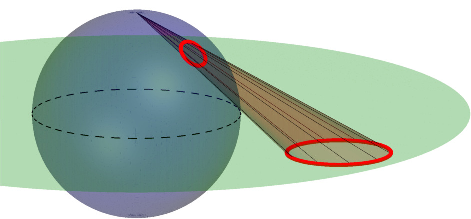
\includegraphics{complex-stereocircle}\qquad 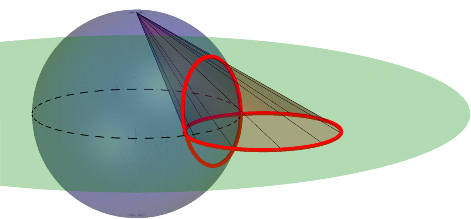
\includegraphics{complex-stereocircle2}
\end{center}

\paragraph{Example}
Given the circle $(x-7)^2+(y+2)^2=49$ in the plane, we inverse project to the sphere: writing $x=\frac X{1-Z}$, $y=\frac Y{1-Z}$ and recalling that $X^2+Y^2+Z^2=1$ we find
\begin{align*}
49&=\frac 1{(1-Z)^2}(X^2+Y^2)+\frac 2{1-Z}(2Y-7X)+49+4\\
&=\frac 1{(1-Z)^2}(1-Z^2)+\frac 2{1-Z}(2Y-7X)+49+4\\
&=\frac 1{1-Z}(1+Z+4Y-14X)+49+4\\
&\implies 14X-4Y+3Z=5
\end{align*}
The inverse projection of the circle lies in the intersection of a plane and the sphere: it is therefore a circle in $S^2$.\\

The study of stereographic projection leads to all manner of funky topics. For more of a taste, you can do a lot worse than to watch this \href{https://www.youtube.com/watch?v=pWOMDm6ejlw}{video.}